\StartPlate{V24}{The equal-capacity test is sharp}{One spare quadratic plane removes the free Arf obstruction, not every attachment constraint.}
\begin{center}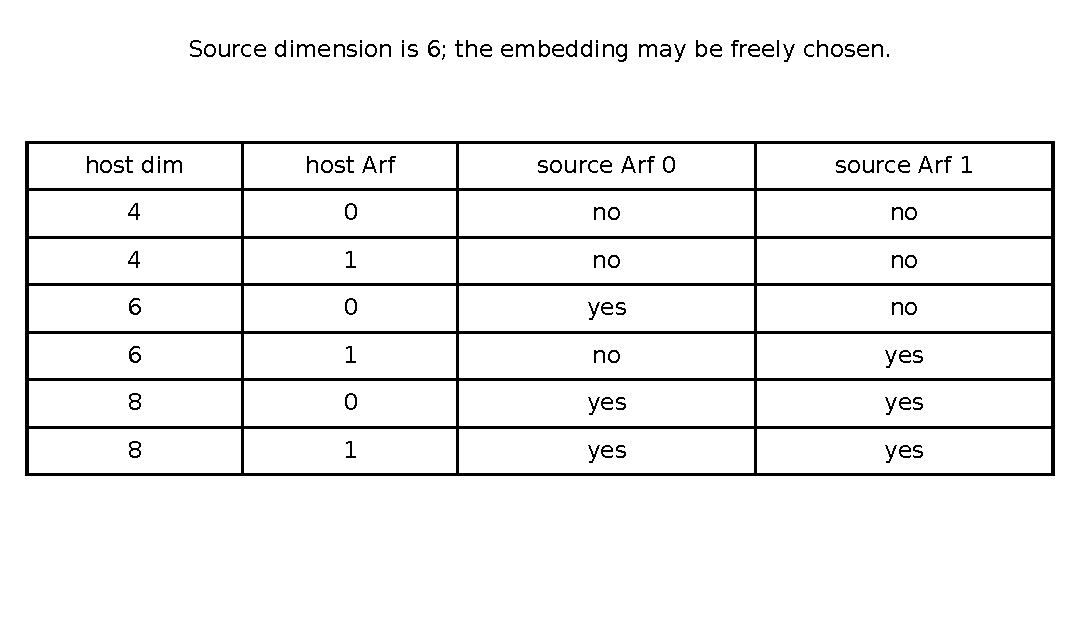
\includegraphics[width=\linewidth]{figures/V24.pdf}\end{center}
Fix a nondegenerate source of dimension six. The table varies the host dimension and its supplied Arf invariant. The embedding may be freely chosen. A four-dimensional host cannot contain the source. At dimension six, the map is an isometry and the Arf signs must agree. At dimension eight, the complementary plane can have either sign.
\[
\operatorname{Arf}(U)
=\operatorname{Arf}(W)+\operatorname{Arf}(V)
\quad\text{for }W\simeq V\perp U.
\]
This is the finite classification argument, not a numerical search over arithmetic matrices. It combines with the original full dyadic capacity formula to isolate the rank-eight equality case.

The word ``free'' matters. A prescribed depth placement, an already fixed quotient embedding, or a stabilizer-equivariance condition may forbid the required change of subspace. The table assumes the actual quadratic host has been supplied. It does not compute that host's native marking, choose its lifts, or authorize modifications to the transport diagram.
\vfill\PlateSource{Finite classification criterion}{Part III, Section 27.2--27.3}{69}
